\documentclass[12pt]{report}
    \usepackage{url}
    \usepackage{xcolor}
    \usepackage{apacite}
    \usepackage{caption}
    \usepackage{pgfgantt}
    \usepackage{mathptmx} 
    \usepackage{graphicx}
    \usepackage{subcaption}
    \usepackage[nottoc,notlof,notlot]{tocbibind} 
    \renewcommand\bibname{References}            
    \usepackage[a4paper, total={6in, 8in}]{geometry}
   
    \definecolor{tail}{RGB}{26, 188, 156}
    \geometry{margin=1in}
    \parindent0pt  
    \parskip10pt             
    \raggedright   
    \title{Sign language recognition using deep learning}
    \author{ Name: MHD Khaled Maen\\
        Matric No: 1523592 \\ 
        [1.5cm]
        Supervised by\\
        Assoc. Prof. Dr. Amelia Ritahani \\}  
    \begin{document}
    \maketitle
    \pagenumbering{roman}                   
    \setcounter{page}{2}                    
    \tableofcontents
    \newpage
    \pagenumbering{arabic}
    \chapter{Introduction} 
        \section{Background}
            \paragraph{}
                Communication is a process of sending and receiving data among individuals. 
                People communicate with o with a considerable measure of ways yet the best way is eye to eye correspondence.
                Numerous individuals trust that the significance of communication 
                is like the importance of breathing. Indeed, communication facilitates the spread of knowledge
                and structures connections between individuals.
            
                Deep learning added a immense lift to the already rapidly developing field of computer vision.
                With deep learning, a lot of new utilization of computer vision techniques have been presented
                and they are currently ending up some portion of our regular day to day existence.
            
                Alongside  with  the intensity of the present computers, there are now various algorithms that were developed 
                to empower the computers to perform tasks such as object tracking and pattern recognition. 
                
                In this study, the attention will be on hand gestures detection and make an interpretation of them into voice.

        \section{Problem Statement}
            \paragraph{}
                Communication difficulties arising from damage to hearing
                directly have an effect on the standard of life. Difficulties in communication could
                end in deviations within the emotional and social development which
                will have a major impact on the standard of lifetime of every one.
                It is well recognized that hearing is crucial to speech and language development, communication, and learning.
                Folks with listening difficulties due to hearing loss or auditory processing problems
                continue to be an under-identified and under-served population. The
                earlier the matter is known and intervention began, the less
                serious the ultimate impact \cite{Frajtag12017}.

                The communication between hearing-impaired and other individuals is a colossal gab 
                need to be filled up. In order to overcome this challenge 
                many researches and products have been developed to solve this problem, 
                but there is a lot to be enhanced.
        
        \section{Objectives}
            \begin{itemize}
                \item To study sign language gestures.
                \item To develop a new hand gesture into voice algorithm.
                \item To construct a hand gesture into voice model.
            \end{itemize}
        
        \section{Scope}
            \paragraph{}
                This research aims to develop a sign language recognition algorithm,
                and converting it into voice.
        \section{Significance}
            \paragraph{}
                Help the hearing-impaired community to communicate with hearing ones, 
                in order to make a strong connected community.

        \section{Timeline}
            \begin{center}
                \begin{ganttchart}[
                    expand chart=\textwidth,
                    bar/.append style={draw=none, fill=tail},
                    hgrid style/.style={draw=black!5, line width=.75pt},
                    vgrid={*1{draw=black!5, line width=.75pt}},
                    ]{1}{14}
                    \gantttitle{Week}{14} \\
                    \gantttitlelist{1,...,14}{1} \\
                    \ganttbar{Title Selectin}{1}{3}  \\
                    \ganttbar{Overall System Review}{2}{7}  \\
                    \ganttbar{Literature Review}{4}{12}  \\
                    \ganttbar{System Design}{8}{11}  \\
                    \ganttbar{Design \& Prototype}{9}{12}  \\
                    \ganttbar{Simulation}{7}{13}  \\
                    \ganttbar{Report Writing}{5}{13}  \\
                    \ganttbar{Submission}{13}{13}  \\
                \end{ganttchart}
            \end{center}
    \chapter{Literature review}
        \section{Introduction}
            \paragraph{}
                This chapter includes reviews of other previous researcher
                and their proposed methods they used in implementing deep learning
                to recognize hand gestures. These researches will help to grasp the knowledge
                to achieve the project's objectives. 
                
        \section{Previous works}
            \paragraph{}
                \cite{Bao2017}, proposed a Deep convolutional neural network algorithm for hand-gesture 
                recognition without hand localisation, since the hands only occupy about 10\% of 
                the image. They used a combination of 9 convolution layers, 3 fully connected layers, 
                interlaced with ReLU(Rectified Linear Unit) and dropout layers as shown in 
                figure \ref{fig:tiny_architecture}. Alongside this architecture the apply some image 
                processing techniques to have sufficient computation efficiency and memory requirement.
                According to the paper the accuracy achieved was 97.1\% in the images with simple backgrounds
                and 85.3\% in the images with complex backgrounds.However, the main disadvantage of of 
                the proposed algorithm is the training set which only includes 7 different gestures,
                and it tends to have bad accuracy with complex backgrounds.
             
                    \begin{figure}
                        \centering
                        \begin{subfigure}[a]{0.5\textwidth}
                          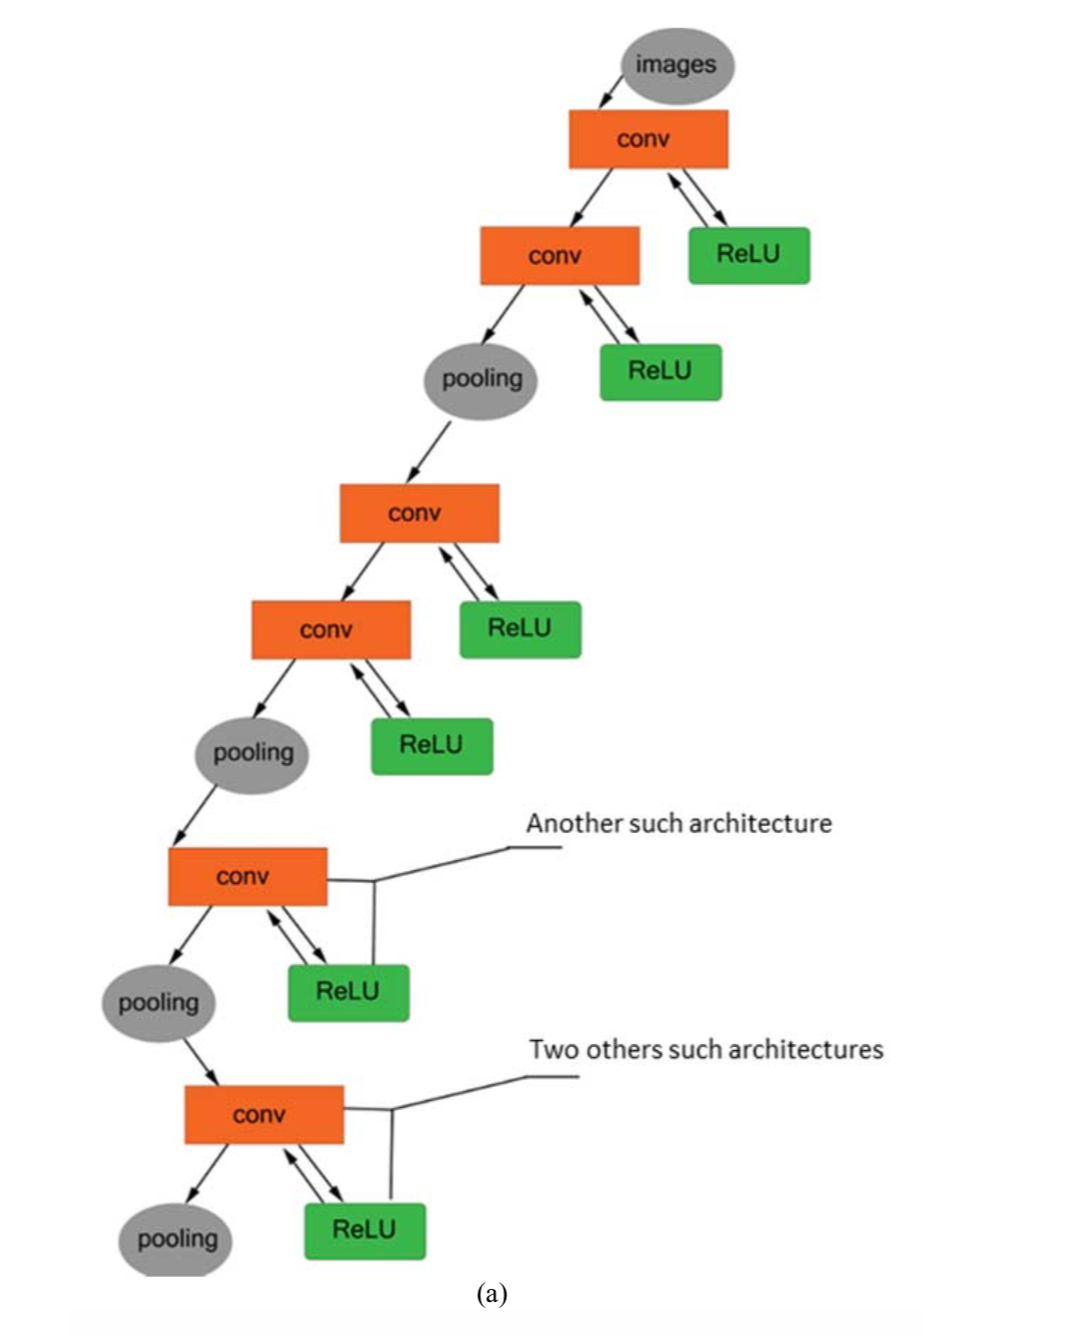
\includegraphics[width=\textwidth]{./images/tiny_a.png}
                        \end{subfigure}
                        \begin{subfigure}[b]{0.3\textwidth}
                            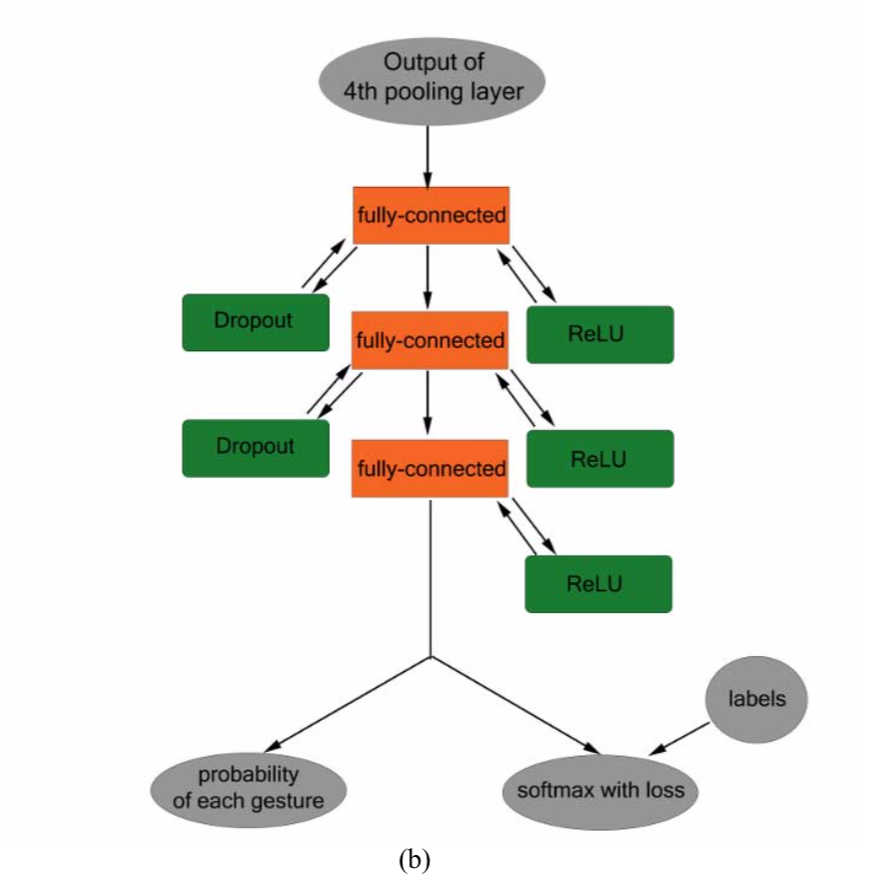
\includegraphics[width=\textwidth]{./images/tiny_b.png}
                        \end{subfigure}
                        \caption{Architecture of the proposed deep CNN }\label{fig:tiny_architecture}
                    \end{figure}

                \newpage

            \paragraph{}
                \cite{Rao2018}, proposed a CNN architecture for classifying selfie sign language gestures. 
                The CNN architecture is designed with four convolutional layers. Each convolutional 
                layer with different filtering window sizes as shown in figure \ref{fig:selfie}  
                They had a dataset with five different subjects performing 200 signs in 5 different viewing angles 
                under various background environments. Each sign occupied for 60 frames or images in a video.
                The proposed model performed training on 3 batches to test the robustness of different training mode 
                using caffe deep learning framework. However, the result accuracy was 92.88\% need more training and improvements. 
    
                    \begin{figure}[h]
                        \centering
                        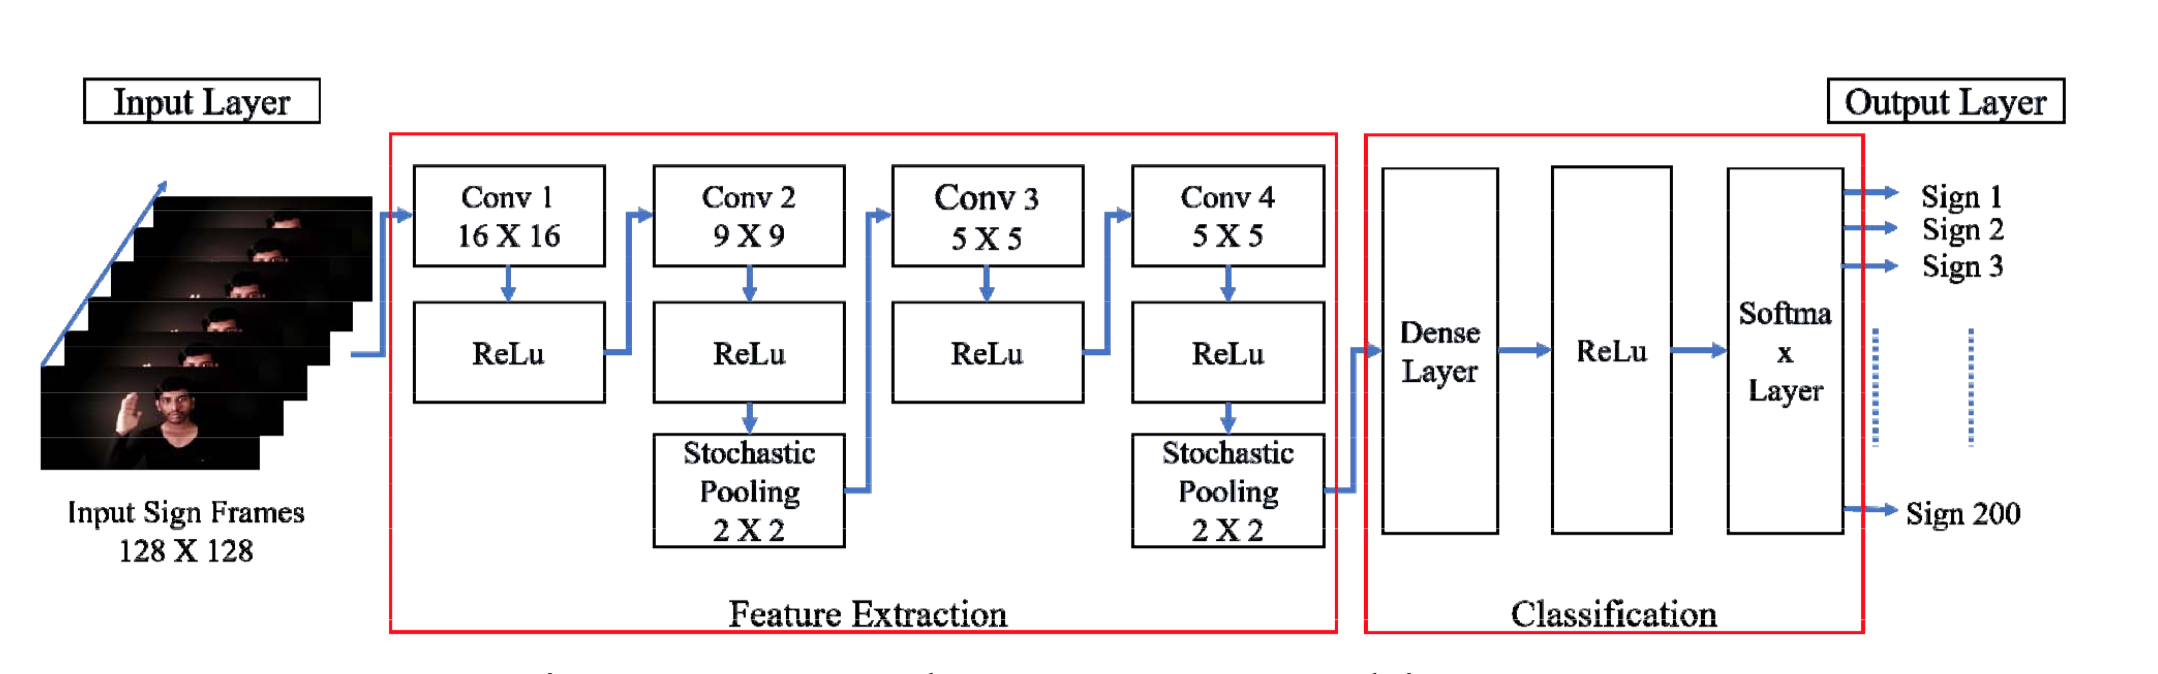
\includegraphics[width=\textwidth]{./images/selfie.png}
                        \caption{Proposed Deep CNN architecture}
                        \label{fig:selfie}
                    \end{figure}

                 \newpage
            
            \paragraph{}
                \cite{Hussain2017}, introduced a CNN based classifier  trained through the process of transfer learning
                over a pretrained convolutional neural network which is trained on a large dataset.
                We are using VGG16 figure \ref{fig:vgg16} as the pretrained model.
                The According to the paper the accuracy was 93.09\%,while using AlexNet 
                figure \ref{fig:alexnet} was 76.96\%. the same problem here with the other papers 
                which is the small number of sign that begin trained on 7 signs, and the accuracy
                need to be improved as well.

                    \begin{figure}[h]
                        \centering
                        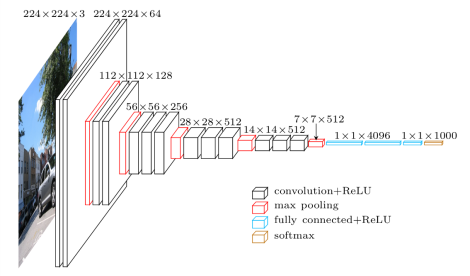
\includegraphics[width=\textwidth]{images/vgg16.png}
                        \caption{VGG16 architecture. Retrieved from www.cs.toronto.edu}
                        \label{fig:vgg16}
                    \end{figure}
                    \begin{figure}[h]
                        \centering
                        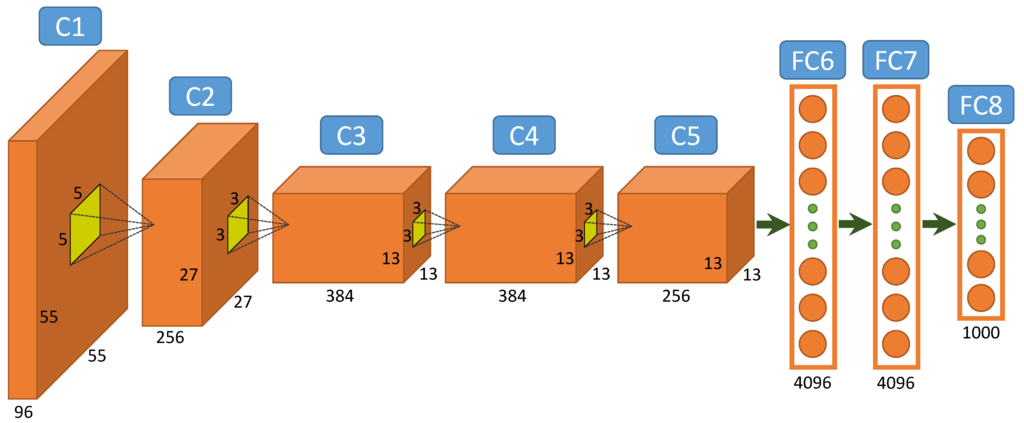
\includegraphics[width=\textwidth]{images/alexnet.png}
                        \caption{VGG16 architecture. Retrieved from www.saagie.com}
                        \label{fig:alexnet}
                    \end{figure}

                \newpage

            \section{Summary}
                \paragraph{}
                    This chapter illustrates some works have been done previously on
                    hand gesture and sign language recognition using deep learning.
                    Table \ref{table:summary} the Summary of the literature review.
                    
                    \begin{center}
                        \begin{table}[h]
                            \caption{Summary of the literature review}
                            \begin{tabular}{ |p{7cm}|p{2cm}|p{2cm}|p{3cm}| }
                                \hline
                                Title & Year & Accuracy & Software\\
                                \hline
                                Tiny Hand Gesture Recognition without Localization via a Deep Convolutional Network & 2017 & 97.1\%& CNN \\
                                \hline
                                Deep Convolutional Neural Networks for Sign Language Recognition & 2018 & 92.88\% & CNN \\
                                \hline
                                Hand Gesture Recognition Using Deep Learning & 2017 & 93.09\% & CNN VGG16 \\
                                \hline
                            \end{tabular}
                            \label{table:summary}
                        \end{table}
                    \end{center}
        \newpage

    \chapter{Methodology}
        \section{Introduction}
        \paragraph{}
            Image recognition, voice producing, system design block diagram figure \ref{fig:system_diagram} 
            and the flowchart of the research is presented in details in this chapter.
            
            \begin{figure}[h]
                \centering
                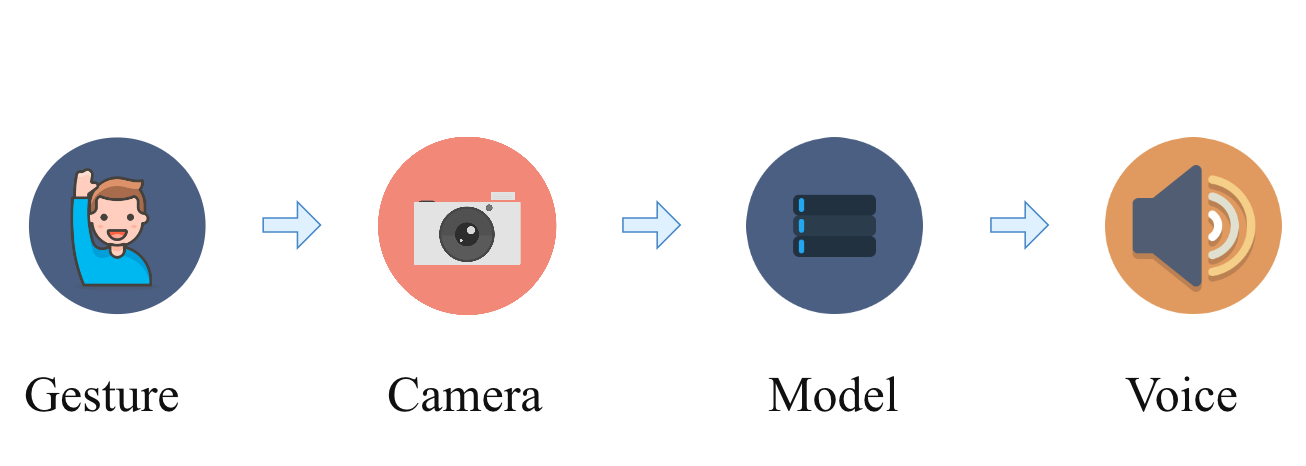
\includegraphics[width=\textwidth]{./images/system_diagram.png}
                \caption{System block diagram}
                \label{fig:system_diagram}
            \end{figure}
        
                    
        \bibliographystyle{apacite}
        \bibliography{scope.bib}
    \end{document}